\documentclass{beamer}
 
\usepackage[utf8]{inputenc}

\usepackage{graphicx}
\usepackage{subfigure}
\usepackage{tikz}
\usetikzlibrary{arrows}

%presentation pre-amble
%The idea behind this file is that it will be used to store all the maths-related macros that I concoct; so that I can import all the commands by \input{this file} in the preamble of any file that I want to use them in.
%This should make the top-level files look a lot cleaner, and the preamble much shorter!

\usepackage{amssymb}
\usepackage{amsmath}
%\usepackage{mathtools}

%begin the macros via newcommand. Try to group them up reasonably!

%standard sets
\newcommand{\naturals}{\mathbb{N}}			%natural numbers
\newcommand{\integers}{\mathbb{Z}}			%integers
\newcommand{\rationals}{\mathbb{Q}}			%rational numbers
\newcommand{\reals}{\mathbb{R}}				%real numbers
\newcommand{\complex}{\mathbb{C}}			%complex numbers

%brackets and norms
\newcommand{\bracs}[1]{\left( #1 \right)}				%encloses input in brackets
\newcommand{\sqbracs}[1]{\left[ #1 \right]}				%encloses input in square brackets
\newcommand{\clbracs}[1]{\left\{ #1 \right\}}			%encloses input in curly bracers
\newcommand{\abs}[1]{\lvert #1 \rvert}					%absolute value
\newcommand{\norm}[1]{\lvert\lvert #1 \rvert\rvert}		%norm 

%function sets
\newcommand{\smooth}[1]{C^{\infty}\bracs{#1}}							%smooth functions
\newcommand{\ltwo}[2]{L^{2}\bracs{#1,\mathrm{d}#2}}						%general L^2 space
\newcommand{\gradSob}[2]{H^1_\mathrm{grad}\bracs{#1, \mathrm{d}#2}}		%gradient Sobolev space
\newcommand{\curlSob}[2]{H^1_\mathrm{curl}\bracs{#1, \mathrm{d}#2}}		%curl Sobolev space
\newcommand{\kSob}[2]{H^1_{k,\mathrm{curl}}\bracs{#1, \mathrm{d}#2}}	%k-curl Sobolev space
\newcommand{\supp}{\mathrm{supp}}										%support of a function

%grad and curl sets
\newcommand{\gradZero}[2]{\mathcal{G}_{ #1, \mathrm{d}#2}\bracs{0}}		%gradients of zero for domain #1 with measure #2
\newcommand{\curlZero}[2]{\mathcal{C}_{ #1, \mathrm{d}#2}\bracs{0}}	%curls of zero for domain #1 with measure #2
\newcommand{\kcurlZero}[2]{\mathcal{C}_{ #1, \mathrm{d}#2}^{(k)}\bracs{0}}	%k-curls of zero for domain #1 with measure #2

%derivatives and grad-like symbols
\newcommand{\diff}[2]{\dfrac{\mathrm{d}#1}{\mathrm{d}#2}}			%complete derivative d#1/d#2
\newcommand{\pdiff}[2]{\dfrac{\partial #1}{\partial #2}}			%partial derivative p#1/p#2
\newcommand{\ddiff}[2]{\dfrac{\mathrm{d}^2 #1}{\mathrm{d}^2 #2}}	%2nd deriv
\newcommand{\grad}{\nabla}											%grad operator
\newcommand{\curl}[1]{\grad^{(#1)}\wedge}							%curl with superscript #1
\newcommand{\kcurl}[1]{\grad_{#1}^{(k)}\wedge}						%k-curl with measure subscript #1

%displaying integrals
\newcommand{\integral}[3]{\int_{#1}#2 \ \mathrm{d}#3}			%integral, domain #1, integrand #2, measure #3
\newcommand{\md}{\ \mathrm{d}}									%differential d

%convergence
%\newcommand{\lconv}[1]{\xrightarrow{#1}}							%convergence with #1 above the rightarrow - requires mathtools
\newcommand{\lconv}[1]{\overset{#1}{\longrightarrow}}				%convergence with #1 above the rightarrow
\newcommand{\toInfty}[1]{ \ \text{as} \ #1 \rightarrow\infty}		%writes out "as #1 tends to infty"

%notation and variable use throughout the file
\renewcommand{\vec}[1]{\mathbf{#1}}				%vectors are bold, not overline arrow
\newcommand{\recip}[1]{\frac{1}{#1}}			%fast reciprocal as a fraction

\newcommand{\dddom}{\widetilde{\Omega}}			%3D domain notation
\newcommand{\ddom}{\Omega}						%2D domain notation
\newcommand{\dddmes}{\widetilde{\mu}}			%3D measure
\newcommand{\ddmes}{\mu}						%2D measure

\newcommand{\graph}{\mathbb{G}}					%graph variable

\usetheme{Madrid}
\usecolortheme{default}
 
%removes figure prefix from captions
\setbeamertemplate{caption}{\raggedright\insertcaption\par} 
 
%Information to be included in the title page
\title{Photonic Fibres from Thin Structures}
\author{William Graham}
\institute{University of Bath}
\date{\today}
 
\begin{document}
 
\frame{\titlepage}
 
%insert a contents or overview slide at the end

%Background 1: Optical Fibres
\begin{frame}
	\frametitle{Optical- vs Photonic Fibres}
	
	\begin{figure}[t]
		\centering
		\includegraphics[width=0.45\textwidth]{Diagrams/Diagram_OpticalFibre.pdf}
		~
		\includegraphics[width=0.45\textwidth]{Diagrams/Diagram_PhotonicFibre.pdf}
	\end{figure}
	\begin{columns}
		\begin{column}{0.45\textwidth}
			\begin{block}{Optical Fibres}
				\begin{itemize}
					\item Developed $\approx 1970$
					\item Light guidance by TIR
				\end{itemize}
			\end{block}
		\end{column}
		\begin{column}{0.45\textwidth}
			\begin{block}{Photonic Fibres}
				\begin{itemize}
					\item Developed $\approx 1980$
					\item Photonic crystal geometry induces "frequency gaps"
				\end{itemize}
			\end{block}
		\end{column}
	\end{columns}
\end{frame} 

%Background 2: Objectives and modelling assumptions
\begin{frame}
	\frametitle{Project Motivation}
		
	
	\begin{block}{Objectives}
	Given a photonic fibre design, determine the frequencies it confines to the hollow cores.
		\begin{enumerate}
			\item Decide on modelling assumptions
			\only<1>{
			\item Determine a suitable mathematical formulation of the problem
			\item Develop a numerical scheme for applications
			}
		\end{enumerate}
	\end{block}
	
	\only<2-3>{
	\begin{block}{Cross section is an infinite periodic sheet}
		\textbf{Justify:} Pattern periodicity $<<$ fibre-cross section width. \newline
		\textbf{Reason:} Gelfand transform - study to family of problems on the unit cell
	\end{block}
	}
	\only<3>{
	\begin{block}{Photonic crystal is infinitely thin}
		\textbf{Justify:} Crystal structure $<$ pattern periodicity. \newline
		\textbf{Reason:} ``Quantum graphs" framework
	\end{block}
	}

\end{frame}

%Theory 1: Quantum Graphs
\begin{frame}
	\frametitle{Quantum Graphs}
	
	\only<1-2>{
		\begin{block}{A Quantum Graph}
			A Quantum Graph (QG) is a finite graph $\graph = \bracs{V,E}$ for a set of vertices $\clbracs{v_{j}}$ and directed edges $I_{jk}=\bracs{v_j, v_k}$ , where:
			\begin{itemize}
				\item Each $I_{jk}\in E$ is associated with an interval $\subset\reals$, which we also call $I_{jk}$.
			\end{itemize}
	For $I_{jk}\in E$, we call $v_j$ the ``left vertex" of $I_{jk}$ and $v_k$ the ``right vertex".
		\end{block}
	}
	
	\only<1>{
	\begin{figure}
		\centering
		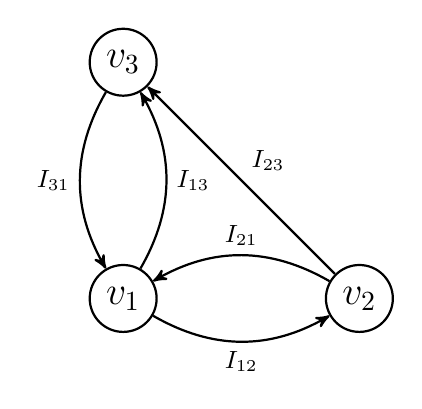
\begin{tikzpicture}[->,>=stealth',auto,node distance=3cm,thick,main node/.style={circle,draw,font=\sffamily\Large\bfseries}]
		\node[main node] (1) {$v_{1}$};
		\node[main node] (2) [right of=1] {$v_2$};
		\node[main node] (3) [above of=1] {$v_3$};
		
		\path[every node/.style={font=\sffamily\small}]
		    (1) edge[bend right] node[anchor=north] {$I_{12}$} (2)
		    (2) edge[bend right] node[anchor=south] {$I_{21}$} (1)
		    (2) edge node[anchor=south west] {$I_{23}$} (3)
		    (3) edge[bend right] node[anchor=east] {$I_{31}$} (1)
		    (1) edge[bend right] node[anchor=west] {$I_{13}$} (3);
		\end{tikzpicture}
	\end{figure}
	}
	
	\only<2>{
	Define 
	\begin{align*}
		L^2\bracs{\graph} &:= \bigoplus_{j\sim k} L^2\bracs{I_{jk}}, \quad
		H^2\bracs{\graph} := \bigoplus_{j\sim k} H^2\bracs{I_{jk}} \\
		\mathcal{D}\bracs{\graph} &:= \clbracs{u \in H^2\bracs{\graph} \ \vert \ u \text{ is continuous at every } v_j\in V}
	\end{align*}
	Characterise functions by their edge-wise forms, $u_{jk} := u\vert_{jk}$.
	}
	
	\only<3-4>{
	Define differential operators by their ``edge-wise action plus ``boundary conditions" at the vertices:
	\begin{align*}
		\mathcal{A} &= \ddiff{}{x} \quad\text{``edgewise"}, \\
		\mathrm{dom}\mathcal{A} &= \clbracs{u\in\mathcal{D}\bracs{\graph} \ \vert \ \text{matching conditions on } u}
	\end{align*}
	We will be interested in Kirchoff-like matching conditions:
	\begin{align*}
		\quad \sum_{j\sim k}u_{jk}'\bracs{v_{k}} = 0
	\end{align*}
	}
	
	\only<4>{
		\textbf{Note:} Quantum Graphs framework is much more general than this!
	}
\end{frame}
%when talking about this slide on the day, you should mention that this is a SUBSET of what you can actually do with quantum graphs!

%Theory 2: Quantum Graphs + M-matrix
\begin{frame}
	\frametitle{Help from Boundary Triples}

	\begin{block}{Dirichlet and Neumann maps}
		$\Gamma_0, \Gamma_1 : \mathrm{dom}\mathcal{A} \rightarrow \complex^{\abs{V}}$,
		\begin{itemize}
			\item Dirichlet map $\bracs{\Gamma_0 u}_j = u\bracs{v_j}$. Sends $u$ to it's Dirichlet data.
			\item Neumann map $\bracs{\Gamma_1 u}_j = \sum_{j\sim k}u_{jk}'\bracs{v_j}$. Sends $u$ to it's Neumann data.
		\end{itemize}
	\end{block}
	
	\begin{block}{	(Weyl-Titchmarsh) M-matrix}
		\begin{align*}
			M\bracs{\omega} &:\complex^{\abs{V}} \rightarrow\complex^{\abs{V}}, \text{ such that } \\
			M\bracs{\omega} &\Gamma_0 u = \Gamma_1 u \quad
			\text{whenever } u\in\mathrm{ker}\bracs{\mathcal{A}-\omega^2}, \ \omega^2\in\complex
		\end{align*}
		Eigenvalues of $\mathcal{A}$ occur at $\omega^2$ such that $\mathrm{det}\bracs{M\bracs{\omega}}=0$
	\end{block}

	\textbf{Key point}: QG eigenvalue problem $\rightarrow$ matrix eigenvalue problem.
	Computers can solve the latter!
\end{frame}

%Theory 3: Motivate the variational formulation
\begin{frame}
	\frametitle{Fibres to Quantum Graphs}
	
	\only<1->{
		\textbf{Key question:} How can we turn a wave-propagation problem for a 3D (singular) photonic fibre into an (essentially 1D) QG problem?
	}
	
	\only<1->{
		\begin{block}{Our domain}
			\only<1>{
				3D space with directions $\bracs{x_1,x_2,x_3}$:
				\begin{figure}
					\centering
					\includegraphics[scale=0.75]{Diagrams/Diagram_Domain3DOutline.pdf}
					~
					\includegraphics[scale=0.55]{Diagrams/Diagram_Domain3DPeriodCell.pdf}
				\end{figure}
				}
				\only<2->{
					\textbf{Our domain is a union of planes, in 3D space!} \newline
					How \textit{can} we understand 3D-differential equations like
					\begin{align*}
						-\grad^2 u = c^2 \dfrac{\partial^2 u}{\partial t^2}
					\end{align*}
					with ``boundary data" involving normal derivatives
					\begin{align*}
						\dfrac{\partial u}{\partial n} = 0?
					\end{align*}
			}
		\end{block}
	}
	
	\only<2->{
		\textbf{Ideas:} 
		\begin{itemize}
			\item Translation invariance $\rightarrow$ use Fourier transform
			\item Use a variational formulation
		\end{itemize}
	}
\end{frame}

%Theory 4: Setup for variational formulation
\begin{frame}
	\frametitle{A variational formulation}
	
	\only<1-2>{
		Fourier transform reduces 3D problem to a 2D problem in the cross-section. \newline
		$\rightarrow$ Consider a 2D construction for now.
	}
	
	\begin{block}{Singular Structure as a Graph}
		\only<1>{
			$\ddom\subset\reals^2$ bounded. \newline
			Let $\graph=\bracs{V,E}$ be a graph embedded into $\ddom$:
			\begin{itemize}
				\item Each $v_j\in V$ is associated to a point $v_j\in\ddom$
				\item Each $I_{jk}\in E$ is associated to the segment $\sqbracs{v_j,v_k}$
			\end{itemize}
		}
		\only<2-3>{
			\begin{columns}
				\begin{column}{0.45\textwidth}
					Let $\lambda_{jk}$ be the 2D singular (Borel) measure that supports 1D Lebesgue measure on $I_{jk}$. \newline
					
					Let $\ddmes$ be the 2D singular (Borel) measure that supports 1D Lebesgue measure on $\graph$:
					\begin{align*}
						\ddmes\bracs{B} &= \sum_{j\sim k}\lambda_{jk}\bracs{B}, \quad B\in \mathcal{B}_{\ddom}
					\end{align*}
				\end{column}
				\begin{column}{0.5\textwidth}
					\begin{figure}
						\centering
						\includegraphics[scale=0.75]{Diagrams/Diagram_SingularMeasure.pdf}
					\end{figure}
				\end{column}
			\end{columns}				
		}
	\end{block}
	
	\only<3>{
		\textbf{Plan:} Do ``calculus" with respect to $\ddmes$? 
	}
\end{frame}

%Theory 5: mu-Sob spaces and gradients of 0
\begin{frame}
	\frametitle{$\gradSob{\ddom}{\mu}$}
	
	\only<1-2>{
		\begin{block}{Constructing ``Sobolev spaces"}
			Let $W$ be the closure of $	\clbracs{\bracs{\phi, \grad\phi} \ \vert \ \phi\in\smooth{\ddom}}$ in $\ltwo{\ddom}{\ddmes}$. \newline
			Then define
			\begin{align*}
				\gradSob{\ddom}{\mu} = \clbracs{u \ \vert \ \bracs{u,z}\in W}.
			\end{align*}
			We \textit{want to} denote the component $z$ in $\bracs{u,z}\in W$ by $\grad_{\ddmes}u$, but...
		\end{block}
	}
	
	\only<2>{
		If $\bracs{u,z_1},\bracs{0,z_2}\in W$ then $\bracs{u,z_1+z_2}\in W$ too! \newline
		$\rightarrow$ $\grad_{\ddmes}u$ is not unique! \newline
		
		We must study the set of ``gradients of zero", $\gradZero{\ddom}{\ddmes}$.
	}
\end{frame}

%Theory 6: gradients of zero
\begin{frame}
	\frametitle{$\gradZero{\ddom}{\ddmes}$}
	
	The best we can do is decompose gradients of functions in $\gradSob{\ddom}{\ddmes}$:
	\begin{block}{Tangential Gradient}
		\begin{itemize}
			\item Every $u\in\gradSob{\ddom}{\ddmes}$ has a unique $\grad_{\ddmes}u\in\ltwo{\ddom}{\ddmes}^2$ such that $\grad_{\ddmes}u \perp \gradZero{\ddom}{\ddmes}$.
			\item Every $\bracs{u,z}\in W$ can be represented as $\bracs{u,\grad_{\ddmes}u + \widetilde{z}}\in W$ for $\widetilde{z}\in\gradZero{\ddom}{\ddmes}$.	
		\end{itemize}
		$\grad_{\ddmes}u$ is the tangential gradient of $u$.
	\end{block}	
	
	\only<2>{
		Where did this come from?
		\begin{itemize}
			\item $\gradZero{\ddom}{\ddmes}$ is a linear subspace of $\ltwo{\ddom}{\ddmes}^2$
			\item For $\bracs{u,z}\in W$, the problem $z+c\perp\gradZero{\ddom}{\ddmes}$ has a unique solution for $c\in\gradZero{\ddom}{\ddmes}$
			\item Then $\grad_{\ddmes}u$ must coincide with this $z+c$, for the solution $c$.
		\end{itemize}
	}
\end{frame}

%Theory 7: some variational equations
\begin{frame}
	\frametitle{A variational formulation}
	
	\only<1>{
		We interpret problems like
		\begin{align*}
			-\grad_{\ddmes}^2 u &= f
		\end{align*}
		in the variational sense:
		\begin{align*}
			\integral{\ddom}{\grad_{\ddmes}u \cdot \grad\phi}{\ddmes} &= \integral{\ddom}{f\phi}{\ddmes}, \quad \forall\phi\in\smooth{\ddom}
		\end{align*}
		\begin{itemize}
			\item Solution is a \textit{pair} $\bracs{u,\grad_{\ddmes}u}$, $u\in\gradSob{\ddom}{\ddmes}$.
			\item $\grad_{\ddmes}u$ can be shown to be \textit{the} aforementioned tangential gradient.
		\end{itemize}
	}
	
	\only<2>{
		What about eigenvalue problems
		\begin{align*}
			-\grad_{\ddmes}^2 u &= \omega^2 u?
		\end{align*}
		Similar interpretation:
		\begin{align*}
			\integral{\ddom}{\grad_{\ddmes}u \cdot \grad\phi}{\ddmes} &= \omega^2\integral{\ddom}{u\phi}{\ddmes}, \quad \forall\phi\in\smooth{\ddom}
		\end{align*}
		\begin{itemize}
			\item $\ddom$ bounded - point spectrum
			\item Can interpret in an operator setting on $\gradSob{\ddom}{\ddmes}$.
		\end{itemize}
	}
	
	\only<1-2>{
		\begin{block}{To solve a problem...}
			\begin{itemize}
				\item Characterise $\gradZero{\ddom}{\ddmes}$
				\item Employ edge-wise structure of $\ddmes$ to get a problem on $\graph$
				\item Study the resulting QG problem!
			\end{itemize}
		\end{block}
	}
\end{frame}

%Example 1: scalar-case wave equation
\begin{frame}
	\frametitle{Working everything through:}
	
	\only<1>{
		\begin{block}{Recall}
			\begin{itemize}
				\item $\ddom\subset\reals^2$ bounded
				\item $\graph=\bracs{V,E}$ a graph embedded into $\ddom$
				\item $\ddmes$ supports 1D Lebesgue measure on $\graph$
			\end{itemize}
		\end{block}
		
		\begin{block}{Characterise $\gradZero{\ddom}{\ddmes}$}
			\begin{enumerate}
				\item Characterise $\gradZero{\ddom}{\lambda_{jk}}$ when $I_{jk}$ is parallel to the $x_1$-axis
				\item Characterise $\gradZero{\ddom}{\lambda_{jk}}$ by applying a rotation to the previous result
				\item Appeal to edge-wise nature of $\gradSob{\ddom}{\ddmes}$ to characterise $\gradZero{\ddom}{\ddmes}$
			\end{enumerate}
		\end{block}
	}
	
	\only<2-3>{
		\begin{figure}
			\caption{Illustration of $\gradZero{\ddom}{\lambda_{jk}}$:}
			\centering
			\includegraphics[scale=1.0]{Diagrams/Diagram_GradZeroEdge.pdf}
		\end{figure}
	}
	
	\only<2>{
		Formally:
		\begin{align*}
			f\in\gradZero{\ddom}{\lambda_{jk}} \Leftrightarrow \exists \phi_n\in\smooth{\ddom} \text{ s.t. } \phi_n\lconv{\ltwo{\ddom}{\lambda_{jk}}}0, \grad\phi_n\lconv{\ltwo{\ddom}{\lambda_{jk}}^2}f
		\end{align*}
		
		\begin{itemize}
			\item Choosing $\phi_n = x_2 f_2$, means $\phi_n\lconv{\ltwo{\ddom}{\lambda_{jk}}}0, \quad \grad\phi_n\lconv{\ltwo{\ddom}{\lambda_{jk}}^2}\bracs{0,f_2}^{\top}$
			\item If $\bracs{f_1,0}^{\top}\in\gradZero{\ddom}{\lambda_{jk}}$, write $L^2$-norms as integrals and change variables to deduce that $f_1=0$
			\item Extend to non-smooth $f$ by density of $\smooth{\ddom}$ in $\ltwo{\ddom}{\lambda_{jk}}$
		\end{itemize}	
	}
	
	\only<3>{
		This implies
		\begin{align*}
			\gradZero{\ddom}{\lambda_{jk}} = \clbracs{\bracs{0,f_2}^{\top} \ \vert \ f_2\in\ltwo{\ddom}{\lambda_{jk}}}
		\end{align*}
		So the tangential gradient
		\begin{align*}
			\grad_{\lambda_{jk}}u &= \bracs{v_1,0}^{\top}, \quad \text{for some } v_1\in\ltwo{\ddom}{\lambda_{jk}}
		\end{align*}
	}
\end{frame}

%Example 2: scalar-wave equation on one edge
\begin{frame}
	\frametitle{Variational formulation}
	
	\only<1>{
		So now consider
		\begin{align*}
			-\grad_{\lambda_{jk}}^2u = \omega^2 u, \quad u\in\gradSob{\ddom}{\lambda_{jk}}
		\end{align*}
		interpreted as
		\begin{align*}
			\integral{\ddom}{\grad_{\lambda_{jk}}u\cdot\grad\phi - \omega^2 u\phi}{\lambda_{jk}} &= 0, \quad \forall\phi\in\smooth{\ddom}
		\end{align*}
	}
	
	\only<1-2>{	
		Perform some manipulations:
		\begin{align*}
			0 &= \integral{\ddom}{v_1 \partial_1\phi - \omega^2 u\phi}{\lambda_{jk}} &\quad \text{by the form for } \grad_{\lambda_{jk}}u \\
			&= \int_0^{\abs{I_{jk}}}\widetilde{v_1}\partial_t\widetilde{\phi} - \omega^2\widetilde{u}\widetilde{\phi} \ \md t &\quad \text{change variables, along the edge } I_{jk}
		\end{align*}
	}
	
	\only<2-3>{
	$\widetilde{v_1}$ looks like a ``derivative" - this can be formalised. \newline
	If $\widetilde{v_1} \approx \partial_t\widetilde{u}$ then we have
	\begin{align*}
		0 &= \int_0^{\abs{I_{jk}}}\widetilde{v_1}\partial_t\widetilde{\phi} - \omega^2\widetilde{u}\widetilde{\phi} \ \md t,
	\end{align*}
	the weak form of
	\begin{align*}
		-\ddiff{u}{t} = \omega^2 u, \quad t\in\sqbracs{0, \abs{I_{jk}}}.
	\end{align*}
	}
	
	\only<3>{
	\textbf{A Quantum Graph problem!} (On a graph with one edge...)
	}
\end{frame}

%Example 3: scalar-wave equation to QG
\begin{frame}
	\frametitle{Scalar equation:}

	\only<1>{
		What about when $I_{jk}$ is not parallel to the $x_1$-axis? \newline
		Apply a rotation...
		\begin{align*}
			\gradZero{\ddom}{\lambda_{jk}} = \clbracs{f\in\ltwo{\ddom}{\lambda_{jk}}^2 \ \vert \ f\bracs{x}\cdot e_{jk} = 0 \ \forall x\in I_{jk}}
		\end{align*}
		where $e_{jk}$ is the unit vector parallel to $I_{jk}$. \newline
		And the whole of $\graph$?
		\begin{align*}
			\gradZero{\ddom}{\ddmes} = \clbracs{f\in\ltwo{\ddom}{\ddmes}^2 \ \vert \ \forall I_{jk}\in E, f\bracs{x}\cdot e_{jk}=0 \ \forall x\in I_{jk}}
		\end{align*}
	}
	
	\only<2>{
		So when we consider 
		\begin{align*}
			-\grad_{\ddmes}u = \omega^2 u, \quad u\in\gradSob{\ddom}{\ddmes}
		\end{align*}
		we end up with
		\begin{align*}
			0 &= \sum_{I_{jk}\in E}\int_0^{\abs{I_{jk}}}\widetilde{v_{jk}^{(1)}}\partial_t\widetilde{\phi} - \omega^2\widetilde{u_{jk}}\widetilde{\phi} \ \md t
		\end{align*}
	}
	
	\only<3>{
		That is,
		\begin{align*}
			-\ddiff{}{x} &\quad \text{ ``edge-wise"}, \\
			\widetilde{u} &\text{ is continuous at each } v_j\in V, \\
			0 &= \sum_{j\sim k}\widetilde{u_{jk}}'\bracs{v_j} \ \forall v_j\in V
		\end{align*}

	\textbf{It really is a Quantum Graph problem now!}
	}
\end{frame}

%Example 4: Wrap up, back to full space problem, get to numerics.
\begin{frame}
	\frametitle{From start to end:}
	
	Originally:
	\begin{columns}
		\begin{column}{0.20\textwidth}
			\begin{figure}
				\centering
				\includegraphics[scale=0.35]{Diagrams/Diagram_Domain3DOutline.pdf}
			\end{figure}			
		\end{column}
		\begin{column}{0.75\textwidth}
			\begin{itemize}
				\item Eigenvalue equation in an unbounded domain.
				\item Periodic structure in $\bracs{x_1,x_2}$-plane.
				\item Translation invariant in $x_3$.
			\end{itemize}
		\end{column}
	\end{columns}
	
	\begin{block}{Interpretation and transforms}
		\begin{columns}
			\begin{column}{0.20\textwidth}
				\begin{figure}
					\centering
					\includegraphics[scale=0.25]{Diagrams/Diagram_Domain3DPeriodCell.pdf}
				\end{figure}			
			\end{column}
			\begin{column}{0.75\textwidth}
				\begin{itemize}
					\item Fourier transform ``out" $x_3$.
					\item Gelfand transform in $\bracs{x_1,x_2}$, quasimomentum $\theta$.
					\item Family of QG problems, parametrised by $\theta$, on the unit cell's graph.
					\item Union of spectra over $\theta\in(-\pi,\pi]^2$ is spectrum of the original problem.
				\end{itemize}
			\end{column}
		\end{columns}	
	\end{block}
\end{frame}

%Example 5: Numerical results
\begin{frame}
	\frametitle{Numerical Results}
	
	\begin{columns}
		\begin{column}{0.40\textwidth}
			\begin{figure}
				\centering
				\includegraphics[scale=0.45]{Diagrams/Diagram_TFRGraph.pdf}
				\caption{Photonic fibre period cell}
			\end{figure}
			\only<4>{
				We can view the spectrum by creating plots, and export the values to data-files.
			}
		\end{column}
		\begin{column}{0.6\textwidth}
			\only<1-3>{
				On which we have the problem
				\begin{align*}
					-\grad_{\ddmes}^2 u &= \omega^2 u
				\end{align*}		
				(effectively the Fourier variable down the fibre is set to $0$)
			}
			\only<4>{
				\begin{figure}
					\centering
					\includegraphics[scale=0.5]{Images/TFR_Numerical_1stBranch.pdf}
					\includegraphics[scale=0.5]{Images/TFR_Numerical_2ndBranch-Periodicity.pdf}
				\end{figure}
			}
		\end{column}
	\end{columns}
	\only<1>{
		We obtain
		\begin{align*}
			-\bracs{\diff{}{t}-i\theta}^2 &= \omega^2 u, \quad \text{edge-wise}, \\
			\widetilde{u} &\text{ is continuous at each } v_j\in V, \\
			0 &= \sum_{j\sim k}\widetilde{u_{jk}}'\bracs{v_j} \ \forall v_j\in V
		\end{align*}	
	}
	\only<2>{
		We construct the M-matrix for each problem by considering
		\begin{align*}
			M\bracs{\omega,\theta}\Gamma_0 \widetilde{u} = \Gamma_1 \widetilde{u}
		\end{align*}
		when $\Gamma_0 \widetilde{u}$ is set to the $k^{\mathrm{th}}$ canonical unit vector, $\Gamma_1 \widetilde{u}$ is the $k^{\mathrm{th}}$ column of $M\bracs{\omega, \theta}$.
	}
	\only<3>{
		We numerically solve the QG problem for the Dirichlet data $\Gamma_0 \widetilde{u} = e_{k}$, and read off the Neumann data $\Gamma_1 \widetilde{u}$ as the column of $M$. \newline
		Then we numerically solve the eigenvalue problem
		\begin{align*}
			\mathrm{det} M\bracs{\omega,\theta} = 0
		\end{align*}
		for $\omega$, for a mesh of values $\theta\in(-\pi,\pi]^2$.
	}

\end{frame}

%For the future - where do we go from here?
\begin{frame}
	\frametitle{Where next?}
	
	The presented work serves as our motivation and guide for more descriptive models:
	\begin{itemize}
		\item Develop a method to handle vector-valued functions (Maxwell systems in particular)
		\only<2>{
			\begin{columns}
				\begin{column}{0.35\textwidth}
					\begin{itemize}
						\item Definition and analysis of $\curlSob{\ddom}{\ddmes}$
						\item Tangential curls, and ``curls of zero"
						\item Variational formulation and the corresponding reduction to QG
						\item Time-dependence
					\end{itemize}				
				\end{column}
				\begin{column}{0.55\textwidth}
					\begin{figure}
					\includegraphics[scale=0.45]{Diagrams/Diagram_CurlZeroPlane.pdf}
					\end{figure}
				\end{column}
			\end{columns}
		}
		\only<3->{
			\item Further development of the numerical scheme
		}
		\only<4>{
			\begin{itemize}
				\item Analysis of solver methods
				\item Handling of the ``Fourier variable"
				\item Speed and efficiency
			\end{itemize}
		}
		\only<5->{
			\item Analysis: singular-structures as an asymptotic limit of thin-structures
		}
		\only<6>{
			\begin{itemize}
				\item Strengthen the link between the two problems
				\item Reduce complex PDE problems to (relatively) simpler ODE problems
				\item Applications in design of fibres and other waveguides
			\end{itemize}
		}
	\end{itemize}
\end{frame}

%thanks for listening slide, questions ETC
\begin{frame}[allowframebreaks]
	\frametitle{References}
	
	Thank you for your attention.
	
	\begin{block}{Reference grouping}
		\begin{itemize}
			\item Photonic Fibres: Knight \cite{knight2003photonic}
			\item Quantum Graphs: Ershova, Karpenko, Kiselev \cite{ershova2014isospectrality}, Cherednichenko, Ershova, Kiselev \cite{cherednichenko2019time}
			\item Variational Formulation: Zhikov \cite{zhikov2000extension}, Exner, Post \cite{exner2005convergence}
			\item NLEVP Methods: Guttel, Tisseur \cite{guttel2017nonlinear}
		\end{itemize}
	\end{block}
	
	\bibliographystyle{unsrt}
	\bibliography{../master_bib.bib}
\end{frame}

\end{document}
